% arara: xelatex: {synctex: true}
% arara: indent: {overwrite: yes}
\documentclass[]{IMTexam}

\usepackage[python]{IMTtikz}

\DeclareSIUnit{\rotation}{rotação}

\givecredits
\author{Isabella B.}
\USPN{11810773}
\date{}
\lecture{Física I} % disciplina
\lcode{4302111}
\hwtype{Resolução} % o que é
\examname{Lista 3} % prova

\begin{document}

\maketitle

\begin{questions}

	\question
	Um jogador de futebol inexperiente chuta um pênalti a \SI{9}{\meter} do gol, levantando a bola com velocidade inicial de \SI{15}{\meter\per\second}. A altura da trave é de \SI{2.4}{\meter}. Calcule:

	\begin{parts}
		\part a que distância máxima da trave, através do gol, um apanhador
		de bola pode ficar agachado;

		\part a que distância mínima devem ficar os espectadores, para que não
		corram risco nenhum de levar uma bolada.

		\begin{solution}

			\correctspacing
			\begin{multi}
				Montando o diagrama para a situação apresentada, temos
				\begin{gather*}
					v_{0x}=v_0\,\cos\theta\\
					v_{0y}=v_0\,\sin\theta
				\end{gather*}
				sendo, respectivamente, as velocidades iniciais em $ x $ e $ y $.

				Supondo que o jogador levantou a bola à altura da trave, temos, por Torricelli
				\begin{align*}
					0^{2}                     & =v_{0y}^{2}-2g\,\num{2.4}   \\
					\del{v_0\,\sin\theta}^{2} & =\num{4.8}g                 \\
					\envert{v_0\,\sin\theta}  & =\envert{\sqrt{\num{4.8}g}}
				\end{align*}
				assumindo $ v_0\,\sin\theta >0 $
				\begin{align*}
					\sin\theta & =\dfrac{\sqrt{\num{4.8}g}}{v_0}                            \\
					\theta     & =\arcsin{\del{\dfrac{\sqrt{\num{4.8}g}}{v_0}}}=\ang{27.22}
				\end{align*}

				Integrando a aceleração da gravidade com respeito ao tempo, temos que:
				\begin{align*}
					\int -g \dif t & =v_y               \\
					\intertext{fazendo $ v_y=0 $ encontramos o tempo de subida, $ t_s $}
					-g\,t_s+v_{0y} & =0                 \\
					t_s            & =\dfrac{v_{0y}}{g}
				\end{align*}

				\nextcol

				\centerline{\begin{tikzpicture}
						\begin{axis}[
								title={$ y(t)\times x(t) $},
								axis lines=middle,
								every axis x label/.style={at={(current axis.right of origin)},anchor=west},
								every axis y label/.style={at={(current axis.north west)},above right=1mm},
								ylabel={$ y $},
								xlabel={$ x $},
								ytick={0,1,2,3},
								xtick={3,5,...,19},
								xmin=-1,xmax=20,
								ymin=-0.25,ymax=3.5,
							]
							\addplot[black,domain=0:18.66] {(15*15*0.813*x - 9.81*x^2)/(2*15*15*(0.889)*(0.889))};
							\coordinate (O) at (axis cs:0,0);
							\coordinate (Gh) at (axis cs:9,2.4);
							\coordinate (x) at (axis cs:2,0);
							\coordinate (S) at (axis cs:{2*cos(27.22)},{2*sin(27.22)});
						\end{axis}

						\draw[-Latex] (O) -- (S) node[above] {$ v_0 $};
						\draw[-Latex,red] (O) -- (S|-O) node[below] {$ v_{0x} $};
						\draw[-Latex,red] (O) -- node[left] {$ v_{0y} $} (S-|O);

						\draw[dashed] (Gh|-O) -- node[rotate=90,above] {Gol} (Gh) -- (Gh-|O) node[left] {$ \num{2.4} $};

						\pic[draw=black, angle radius=20pt,angle eccentricity=1,"$ \theta=\ang{27.22} $" {xshift=28pt,yshift=2pt}] {angle=x--O--S};
					\end{tikzpicture}}

				Sendo $ v_x(t) $ constante no tempo, temos:
				\begin{align*}
					v_x(t)            & =v_{0x}\implies                                                             \\
					\int v_x(t)\dif t & =\int v_{0x}\dif t\implies                                                  \\
					x(t)              & =v_{0x}t + \cancelto{0}{x_0}                                                \\
					\intertext{para $ t=2t_s $ teremos o tempo de queda, dada a simetria da parábola}
					x(2t_s)           & =v_{0}\cos\theta \,2 \del{\dfrac{v_{0y}}{g}}                                \\
					                  & =v_{0}2\cos\theta \del{\dfrac{v_{0}\sin\theta}{g}}                          \\
					                  & =\dfrac{v_{0}^{2}2\sin\theta\cos\theta}{g}                                  \\
					                  & =\dfrac{v_{0}^{2}\sin{2\theta}}{g}                                          \\
					\intertext{substituindo os valores}
					                  & =\dfrac{15^{2}\sin{2\cdot\ang{27.22}}}{\num{9.81}}\approx\SI{18.66}{\meter}
				\end{align*}
			\end{multi}
		\end{solution}
	\end{parts}

	\question
	Um canhão lança um projétil por cima de uma montanha de altura $ h $, de forma a passar quase tangenciando o cume $ C $ no ponto mais alto de sua trajetória. A distância horizontal entre o canhão e o cume é $ R $. Atrás da montanha há uma depressão de profundidade $ d $ (Fig. \ref{fig:fig1}).

	\begin{figure}[H]
		\centering
		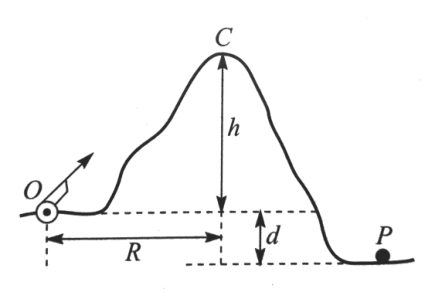
\includegraphics[width=0.7\linewidth]{screenshot001}
		\caption{Canhão lançando um projétil por cima de uma montanha}
		\label{fig:fig1}
	\end{figure}

	Determine a distância horizontal entre o ponto de lançamento $ O $ e o ponto $ P $ onde o projétil atinge o solo, em função de $ R, d $ e $ h $.

	\begin{solution}
		Consideramos a origem o ponto $ O $ de lançamento do projétil, onde posicionaremos um eixo de coordenadas com os eixos $ y $ orientado para cima e $ x $ para a direita.

		Sendo o movimento parabólico uma função quadrática da forma \[ y(x)=a\,x^{2}+b\,x+c \]
		onde $ y $ é o deslocamento vertical e $ x $ é o deslocamento horizontal, derivando ambos os lados, temos
		\begin{align*}
			(y(x))' & =(a\,x^{2}+b\,x+c)' \\
			v_y(x)  & =2a\,x+b
		\end{align*}
		onde $ v_y $ é a projeção da velocidade no eixo $ y $.

		Seja $ v_{0y} $ a velocidade inicial projetada no eixo $ y $, montando dois sistemas com os valores conhecidos para $ v(x) $ e $ y(x) $, respectivamente, temos
		\begin{align*}
			 & \begin{cases}
				v_y(0)=b=v_{0y} \\
				v_y(R)=0\implies 2a\,R+v_{0y}=0\implies a=-\dfrac{v_{0y}}{2R}
			\end{cases}  \\
			 & \begin{cases}
				y(0)=0\implies c=0 \\
				y(R)=h\implies -\dfrac{v_{0y}}{2R}\,R^{2}+v_{0y}\,R=h
			\end{cases}
		\end{align*}
		Resolvendo a última equação para $ v_{0y} $, temos
		\begin{align*}
			-\dfrac{v_{0y}}{2}\,R+v_{0y}\,R & =h \\
			\dfrac{v_{0y}}{2}\,R=h               \\
			v_{0y}=\dfrac{2h}{R}
		\end{align*}

		Portanto, $ y(x)=-\dfrac{v_{0y}}{2R}x^{2}+v_{0y}\,x\implies y(x)=-\dfrac{h}{R^{2}}x^{2}+2\dfrac{h}{R}x $.

		Resolvendo para $ y(x)=-d $, temos
		\begin{align*}
			-\dfrac{h}{R^{2}}x^{2}+2\dfrac{h}{R}x   & =-d \\
			-\dfrac{h}{R^{2}}x^{2}+2\dfrac{h}{R}x+d & =0
		\end{align*}

		\begin{multi}[2][t]

			por Bháskara
			\begin{align*}
				\Delta & =\del{2\dfrac{h}{R}}^{2}-4\del{-\dfrac{h}{R^{2}}}d \\
				       & =\dfrac{4}{R^{2}}h^{2}+\dfrac{4}{R^{2}}h\cdot d    \\
				       & =\dfrac{4}{R^{2}}\del{h^{2}+h\cdot d}
			\end{align*}
			\begin{align*}
				x & =\dfrac{-\dfrac{2h}{R}\pm\sqrt{\dfrac{4}{R^{2}}\del{h^{2}+h\cdot d}}}{2\del{-\dfrac{h}{R^{2}}}}
			\end{align*}

			\nextcol
			como $ x>0 $
			\begin{align*}
				x & =\dfrac{\cancel{\dfrac{2}{R}}h+\cancel{\dfrac{2}{R}}\sqrt{h^{2}+h\cdot d}}{\cancel{\dfrac{2}{R}}\cdot\dfrac{h}{R}} \\
				  & =\dfrac{R}{h}\del{h+\sqrt{h^{2}\del{1+d/h}}}                                                                       \\
				  & =R\del{1+\sqrt{1+\dfrac{d}{h}}}
			\end{align*}
		\end{multi}
	\end{solution}



	\question
	Uma roda maior, de \SI{30}{\centi\meter} de raio, transmite seu movimento à uma menor, de \SI{20}{\centi\meter} de raio, através de uma correia sem fim $ C $, que permanece sempre bem esticada e sem deslizamento. A roda maior, partindo do repouso com aceleração angular uniforme, leva \SI{1}{\minute} para atingir sua velocidade de regime permanente, e efetua um total de 540 rotações durante esse intervalo. Calcule a velocidade angular da roda menor e a velocidade linear da correia uma vez atingido o regime permanente.

	\begin{solution}

		\begin{multi}
			Sendo $ v $ a velocidade linear, $ \omega $ a velocidade angular, $ \alpha $ a aceleração e $ \theta $ uma posição angular\footnote{Ambos problemas de movimento circular nessa lista não lidam com posições absolutas, somente deslocamentos e, portanto, só nos importamos com os $ \Delta\theta $.} ($ \theta=\theta+n\pi,\, n\in \mathbb{Z}$). Denotaremos pelo índice $ m $ as quantidades referentes à roda de raio menor, e usaremos $ M $ para as quantidades relativas à roda maior (por ex.: $ v_m $ é a velocidade linear da roda menor, e $ v_M $ é da roda maior).
			Sejam $ r $ e $ R $ os raios das rodas menor e maior, respectivamente.

			\nextcol

			\centering
			\begin{tikzpicture}[x=1.5cm,y=2cm]
				\node[circle,draw,minimum size=1.5cm] (c1) at (0,0) {};
				\node[circle,draw,minimum size=1.2cm] at (0,0) {};

				\node[circle,draw,minimum size=1cm] (c2) at (3,0) {};
				\node[circle,draw,minimum size=0.8cm] at (3,0) {};

				\draw[-Latex] (0:-1cm) arc (0:-30:-1cm) node[midway,left] {$ \omega_M $};

				\draw[-Latex] (3,0) +(30:0.7cm) arc (30:0:0.7cm) node[midway,right] {$ \omega_m $};

				\coordinate (a) at (0,0.75cm);
				\coordinate (b) at (0,-0.75cm);

				\draw[-Stealth] (0,0) -- node[below,xshift=-5pt] {$ R $} (135:0.6cm);

				\draw[-Stealth] (3,0) -- node[below] {$ r $} +(30:0.4cm);

				\draw (a) -- (tangent cs:node=c2,point={(a)},solution=2) (b) -- (tangent cs:node=c2,point={(b)},solution=1);

				\draw[-Latex] ($ (a)!0.4!(tangent cs:node=c2,point={(a)},solution=2)+(0,0.1) $) -- node[above] {$ v $} ($ (a)!0.6!(tangent cs:node=c2,point={(a)},solution=2)+(0,0.1) $);
			\end{tikzpicture}
		\end{multi}


		Primeiro, devemos encontrar a velocidade angular da roda maior, $ \omega_M $. Para isso, basta integrarmos sua aceleração $ \alpha_M $ (e depois a velocidade) para o intervalo de \SIrange{0}{60}{\second} e igualarmos ao deslocamento:
		\begin{align*}
			\int_{0}^{60}\sbr{\int\alpha_M\dif t}\dif t  & =540\cdot 2\pi                                                 \\
			\int_{0}^{60}\alpha_M\, t\dif t              & =1080\pi                                                       \\
			\eval{\dfrac{1}{2}\alpha_M \,t^{2}}_{0}^{60} & =1080\pi                                                       \\
			\dfrac{1}{2}\alpha_M \cdot 60^{2}            & =1080\pi                                                       \\
			\alpha_M                                     & =\dfrac{2160}{3600}\pi=\SI{0.6\pi}{\radian\per\second\squared}
		\end{align*}
		E, portanto, $ \omega_M=\num{0.6\pi}\cdot60=\SI{36}{\radian\per\second} $. Sendo a velocidade linear das correias igual, temos
		\begin{align*}
			v_m         & =v_M                                                \\
			\omega_m\,r & = \omega_M\,R                                       \\
			\omega_m    & =\dfrac{R}{r}\omega_M                               \\
			\omega_m    & =\dfrac{30}{20}36\pi=\SI{54\pi}{\radian\per\second}
		\end{align*}
		Logo, $ v_m=54\pi\cdot\num{0.2}=\SI{10.8}{\meter\per\second}=v_M=v $.

	\end{solution}



	\question
	Uma roda partindo do repouso é acelerada de tal forma que sua velocidade angular aumenta uniformemente para \SI{180}{\rpm} em \SI{3}{\minute}. Depois de girar com essa velocidade por algum tempo, a roda é freada com desaceleração angular uniforme, levando \SI{4}{\minute} para parar. O número total de rotações é \num{1080}. Quanto tempo, ao todo, a roda ficou girando?

	\begin{solution}
		Sendo a aceleração $ \alpha $ e a desaceleração $ \beta $, encontramos a aceleração $ \alpha $ fazendo:
		\[ \alpha\cdot3=180\implies \alpha=\SI{60}{\rpm\per\minute} \]
		E a desaceleração $ \beta $ por:
		\[ 180-\beta\cdot4=0\implies \beta=\SI{45}{\rpm\per\minute} \]

		Sendo a velocidade angular da roda
		\[
			\omega(t)=\begin{cases}
				\displaystyle\int_0^{t}60\dif \tau          & \text{para }0\leqslant t < \SI{3}{\min}       \\
				180                                         & \text{para }\SI{3}{\min}\leqslant t < t_c     \\
				180+\displaystyle\int_{t_c}^{t}-45\dif \tau & \text{para }t_c\leqslant t < t_c+\SI{4}{\min}
			\end{cases} \]
		onde $ t_c $ é o tempo total em que a roda permanece em velocidade constante.

		Temos que o deslocamento total será igual à integral da velocidade, com cada parcela tomada a parte:
		\begin{align*}
			\int_{0}^{3}\sbr{\int_{0}^{t} 60 \dif \tau}\dif t+\int_{3}^{t_c} 180 \dif t+\int_{t_c}^{t_c+4}180+\sbr{\int_{t_c}^{t} -45 \dif \tau}\dif t & =\num{1080}                         \\
			\int_{0}^{3}60\,t\dif t+\eval{180t}_{3}^{t_c}+\int_{t_c}^{t_c+4}180-45\del{t-t_c}\dif u                                                    & =\num{1080}                         \\
			\intertext{tomando $ u=t-t_c\implies \dif u=\dif t $ na integral da direita, temos}
			\eval{\dfrac{1}{2}60\,t^{2}}_{0}^{3}+180\del{t_c-3}+\int_{0}^{4}180-45u\dif u                                                              & =\num{1080}                         \\
			30\cdot3^{2}+180t_c-540+\eval{\del{180u-\dfrac{1}{2}45\,u^{2}}}_{0}^{4}                                                                    & =\num{1080}                         \\
			180t_c-270+180\cdot4-\dfrac{1}{2}45\cdot4^{2}+                                                                                             & =\num{1080}                         \\
			t_c                                                                                                                                        & =\dfrac{990}{180}=\SI{5.5}{\second}
		\end{align*}
		E, portanto, o tempo total de rotação é $ \num{5.5}+4=\SI{9.5}{\min} $.
	\end{solution}



	\question
	Um bombardeiro, a \SI{300}{\meter} de altitude, voando a \SI{180}{\kilo\meter\per\hour}, mergulha segundo um ângulo de \ang{30} com a horizontal, em perseguição a um carro que viaja a \SI{90}{\kilo\meter\per\hour}. A que distância horizontal do carro deve ser lançada uma bomba para que acerte o alvo?

	\begin{solution}
		Posicionamos nosso eixo de coordenadas com origem na intercessão da posição inicial do avião (na vertical), e da posição do carro (na horizontal), com o eixo $ y $ positivo para cima e o eixo $ x $	positivo para a direção do carro (direita).



		\begin{multi}
			Assumindo que o bombardeiro mergulha e solta a bomba em $ t=0 $, podemos calcular o tempo de queda da bomba $ t_q $, e a partir deste, encontrar a distância desejada $ d $.

			Sendo a velocidade da bomba $ v_b $, a velocidade do avião $ v_a $, a velocidade do carro $ v_c $ e a altura inicial do bombardeiro $ h $, a bomba terá equações de movimento:
			\begin{gather}
				x_b(t)=\int_{0}^{t} v_{ax}\dif \tau,\label{eq:bombX}\\
				y_b(t)=h+\int_{0}^{t} -v_{ay}+\sbr{\int_{0}^{\tau}-g\dif t'}\dif \tau\label{eq:bombY}
			\end{gather}

			\nextcol

			\centering
			\begin{tikzpicture}[x=1cm,y=1cm]
				\draw[->] (-0.25,0) -- (6,0) node[right] {$ x $};
				\draw[->] (0,-0.25) -- (0,3.5) node[above] {$ y $};

				\node[] at (4,0) {
\includegraphics[scale=0.3]{screenshot002}};
				\node[rotate=-30] at (0,3) {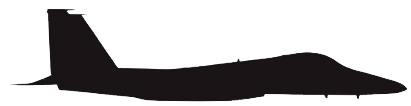
\includegraphics[scale=0.3]{screenshot003}};
				\node[rotate=-30] at (0,2.3) {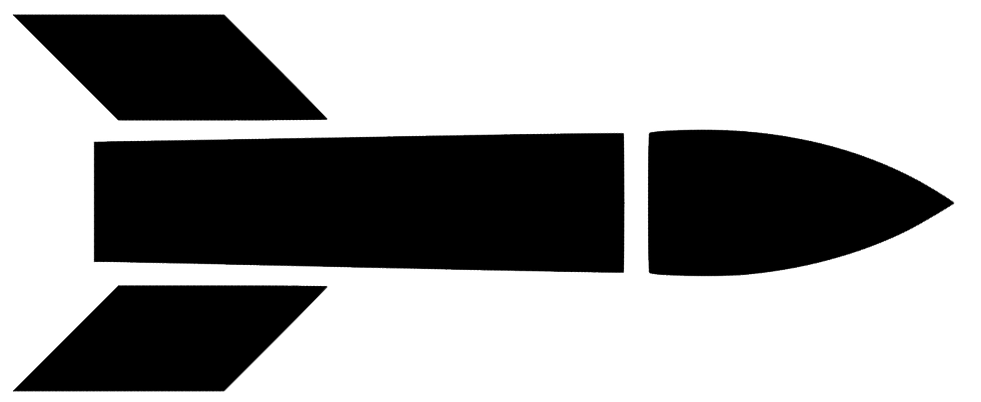
\includegraphics[scale=0.02]{screenshot004}};

				\draw[decorate,decoration={brace,raise=3pt,amplitude=8pt}] (-0.5,0) -- node[rotate=90,yshift=20pt] {\SI{300}{\meter}} (-0.5,2.8);

				\draw[-Latex] (4,0.5) -- node[above] {$ v_c $} +(1,0);

				\draw[-Latex] (0,2.5) -- +(-30:1) node[below] {$ v_a $};

				\draw[decorate,decoration={brace,raise=3pt,amplitude=8pt,mirror}] (0,-0.25) -- node[below=10pt] {$ d $} (4,-0.25);

				\draw[dashed] (0,2.98) coordinate (a) -- +(2,0) coordinate (h);
				\coordinate (p) at ($ (0,2.98)+(-30:1) $);

				\pic[draw=black, angle radius=15pt,angle eccentricity=1,"$ \ang{30} $" {xshift=10pt,yshift=-2pt}] {angle=p--a--h};
			\end{tikzpicture}
		\end{multi}

		onde \ref{eq:bombX} descreve sua posição no eixo $ x $ e \ref{eq:bombY} descreve sua posição no eixo $ y $, e $ v_{ax}=v_a\cos\ang{30}, v_{ay}=v_a\sin\ang{30} $ são as componentes horizontal e vertical velocidade do avião, respectivamente.

		Resolvendo para $ y_b(t)=0 $, temos:
		\begin{align*}
			h+\int_{0}^{t} -v_{ay}-\eval{g\,t'}_{0}^{\tau}\dif\tau       & =0 \\
			h+\int_{0}^{t} -v_{ay}-g\,\tau\dif\tau                       & =0 \\
			h+\eval{\del{-v_{ay}\,\tau-\dfrac{1}{2}g\,\tau^{2}}}_{0}^{t} & =0 \\
			h-v_{ay}\,t-\dfrac{g}{2}\,t^{2}                              & =0
		\end{align*}
		Sendo
		\footnote{Caso tenha dificuldades em entender esse método, \href{https://www.youtube.com/watch?v=MHXO86wKeDY}{esse vídeo} explica bem. Alternativamente, faça por Bháskara.} as raízes da parábola simétricas em relação à seu valor extremo (um máximo, no caso particular), temos:
		\[ \del{h-v_{ay}\,t-\dfrac{g}{2}\,t^{2}}'=0\implies -v_{ay}-g\,t_{max}=0\implies t_{max}=\dfrac{-v_{ay}}{g} \]
		Sendo $ y_b(t) $ um polinômio de segundo grau no formato $ a\,x^{2}+b\,x+c $, com fatoração equivalente $ (x-r_1)(x-r_2) $, temos $ c=-h/2g $.
		Escrevendo as raízes na forma $ t_{max}+d_r $ e $ t_{max}-d_r $s, temos que $ -2h/g $ atende a igualdade
		\[ (t_{max}+d_r)(t_{max}-d_r)=-\dfrac{2h}{g}\implies \del{\dfrac{-v_{ay}}{g}}^{2}-d_r^{2}=-\dfrac{2h}{g}\implies d_r=\sqrt{\del{\dfrac{v_{ay}}{g}}^{2}+\dfrac{2h}{g}} \]
		Portanto, as raízes da função são
		\[ t_{max}\pm d_r=\dfrac{-v_{ay}}{g}\pm\sqrt{\del{\dfrac{v_{ay}}{g}}^{2}+\dfrac{2h}{g}} \]

		E a bomba intercepta o carro com tempo mínimo igual a menor raiz positiva raiz ($ t_{max}+ d_r $).
		Sendo $ x_c(t)=d+\displaystyle\int_{0}^{t}v_c\dif\tau $ a posição do carro, resolvendo $ x_b(t)=x_c(t) $, temos:
		\begin{align*}
			x_b(t)  & =x_c(t)                                                                                                                                                                                                                    \\
			v_{ax}t & =d+v_c\,t                                                                                                                                                                                                                  \\
			\intertext{isolando $ d $ e tomando $ t=t_{max}+ d_r $, temos}
			d       & =\del{t_{max}+ d_r}\del{v_{ax}-v_c}                                                                                                                                                                                        \\
			        & =\del{\dfrac{-v_{a}\sin\ang{30}}{g}+\sqrt{\del{\dfrac{v_{a}\cdot\sin\ang{30}}{g}}^{2}+\dfrac{2h}{g}}}\del{v_{a}\,\cos\ang{30}-v_c}                                                                                         \\
			        & =\del{\dfrac{-50\cdot\num{0.5}}{\num{9.81}}+\sqrt{\del{\dfrac{50\cdot\num{0.5}}{\num{9.81}}}^{2}+\dfrac{2\cdot300}{\num{9.81}}}}\del{50\dfrac{\sqrt{3}}{2}-25}\quad\text{assumindo }g=\SI{9.81}{\meter\per\second\squared} \\
			d       & =50\del{\dfrac{-25+\sqrt{\del{25^{2}+\num{5886}}}}{\num{9.81}}}\del{\sqrt{3}-1}\approx\SI{155.123}{\meter}
		\end{align*}
	\end{solution}

	\clearpage

	\question
	Um rio de \SI{1}{\kilo\meter} de largura tem uma correnteza de velocidade \SI{1.5}{\kilo\meter\per\hour}. Um homem atravessa o rio de barco, remando a uma velocidade de \SI{2.5}{\kilo\meter\per\hour} em relação à água.

	\begin{parts}
		\part Qual o tempo mínimo que leva para atravessar o rio? Onde desembarca nesse caso?

		\begin{solution}
			O tempo mínimo ocorre quando o homem viaja com velocidade $ v_b $ perpendicular à margem do rio e, portanto, leva $ t=\dfrac{1}{\num{2.5}}=\SI{0.4}{\hour} $. Nesse tempo, a corrente do rio o carrega por $ d=\num{0.4}\cdot\num{1.5}=\SI{0.6}{\kilo\meter} $.
		\end{solution}

		\part Suponha agora que o homem quer chegar a um ponto diametralmente oposto na outra margem, e tem duas opções: remar de forma a atingi-lo diretamente, ou remar numa direção perpendicular à margem, sendo arrastado pela correnteza até além do ponto onde quer chegar, e depois caminhar de volta até lá. Se ele caminha a \SI{6}{\kilo\meter\per\hour}, qual das duas opções é mais vantajosa, e quanto tempo leva?

		\begin{solution}
			Pela primeira opção, o homem vai ter q se locomover de tal forma a ter uma velocidade $ v_{b}' $ que forma um ângulo $\theta$ com a correnteza.

			Temos, então \[ v_{b\parallel}'=v_b\cos\del{\theta}=v_c\implies \cos\theta=\dfrac{\num{1.5}}{\num{2.5}}=\num{0.6} \]
			Pela relação fundamental da trigonometria, $ \sin\theta=\sqrt{1-\cos^{2}\theta}=\num{0.8} $, e daí tiramos \[ t_1=\dfrac{1}{v_{b\perp}'}=\dfrac{1}{v_b\sin\theta}=\dfrac{1}{\num{2.5}\cdot\num{0.8}}=\SI{0.5}{\hour} \]
			Como o tempo total $ t_2 $ na situação dois será dado pelo tempo mínimo (encontrado no item anterior) somado do tempo para o homem andar \SI{0.6}{\meter}, temos
			\[ t_t=\num{0.4}+\dfrac{\num{0.6}}{6}=\SI{0.5}{\hour} \]
			E, portanto, ambas opções levam ao mesmo tempo gasto.
		\end{solution}
	\end{parts}



	\question
	As \SI{8}{\hour} da manhã, um navio sai do porto de Ilhéus, rumando para \ang{45}SO, à velocidade de 16 nós (1 nó $ = $ 1 milha marítima por $ = $ \SI{1852}{\meter\per\hour}). À mesma hora, outro navio está \ang{45} NO de Ilhéus, a 40 milhas marítimas de distância, rumando em direção a Ilhéus, a uma velocidade de 12 nós. A que hora os dois navios passam à distância mínima um do outro? Qual é essa distância?

	\clearpage

	\begin{solution}

		\begin{multi}
			Sendo o ângulo entre os navios de \ang{90}, podemos fixar nosso referencial com origem no porto, $ \ihat $ no sentido do navio saindo de Ilhéus e $ \jhat $ no sentido do navio indo para Ilhéus, o que nos dá as seguintes equações de movimento:
			\begin{gather*}
				\vec{r_s}=16t\,\ihat\\
				\vec{r_i}=40-12t\,\jhat
			\end{gather*}
			Sendo a distância entre eles dada por
			\begin{equation}\label{eq:distBoats}
				d=\sqrt{|\vec{r_s}|^{2}+|\vec{r_i}|^{2}}
			\end{equation}

			\nextcol

			\centering

			\begin{tikzpicture}[x=1.5cm,y=1.5cm]
				\begin{scope}[rotate=135]
					\draw[gray] (-0.4,-0.4) grid[xstep=0.5,ystep=0.5] (2.4,2.4);

					\fill[white] (2.4,0) -- (0,2.4) -- (2.4,2.4) -- cycle;

					\draw[-Latex] (0,0) -- node[fill=white,inner sep=0.5pt,above right] {$ \ihat $} (0.5,0);
					\draw[-Latex] (0,0) -- node[fill=white,inner sep=0.5pt,below right] {$ \jhat $} (0,0.5);

					\coordinate (A) at (1.5,0);
					\coordinate (B) at (0,1.5);

					\draw[-Latex] (A) -- node[fill=white,inner sep=0.5pt,above right] {$ \vec{r_s} $} +(0.8,0);
					\draw[-Latex] (B) -- node[fill=white,inner sep=0.5pt,above left] {$ \vec{r_i} $} +(0,-0.6);

					%					\draw[line width=3pt,white,decorate,decoration={brace,raise=3pt,mirror,amplitude=8pt}] (A) -- (B);
					%					\draw[thick,decorate,decoration={brace,raise=3pt,mirror,amplitude=8pt}] (A) -- node[fill=white,inner sep=0.5pt,left=15pt] {$ d $} (B);

					\draw[dashed] (A) -- +(0.6,0.6) (B) -- +(0.6,0.6);
					\draw[] ($ (A)+(0.525,0.525) $) -- +(0.125,0.125) ($ (B)+(0.525,0.525) $) -- +(0.125,0.125);

					\draw[Stealth-Stealth] ($ (A)+(0.6,0.6) $) -- node[fill=white] {$ d $} ($ (B)+(0.6,0.6) $);

					%					\draw[thick,decorate,decoration={brace,raise=3pt,mirror,amplitude=8pt}] ($ (A)+(0.5,0.5) $) -- node[left=10pt] {$ d $} ($ (B)+(0.5,0.5) $);
				\end{scope}

				\filldraw (0,0) circle (1.5pt) node[fill=white,inner sep=0.5pt,right=5pt,text width=1.7cm, align=center] {Porto de Ilhéus};

				\filldraw (A) circle (1.5pt) node[fill=white,inner sep=0.5pt,right=5pt] {Navio saindo};

				\filldraw (B) circle (1.5pt) node[fill=white,inner sep=0.5pt,right=5pt] {Navio indo};


				%				\node 
			\end{tikzpicture}
		\end{multi}

		podemos derivar \ref{eq:distBoats} e igualar a zero para encontrar o ponto extremo desejado.
		\begin{align*}
			\dod{}{t}\sbr{d} & =\del{\sqrt{|\vec{r_s}|^{2}+|\vec{r_i}|^{2}}}'=\del{\sqrt{\del{16t}^{2}+\del{40-12t}^{2}}}' \\
			                 & =\del{\sqrt{256t^{2}+1600-960t+144t^{2}}}'=\del{4\sqrt{5}\sqrt{20-12t+5t^{2}}}'             \\
			                 & =4\sqrt{5}u'\del{u^{1/2}}'\quad\text{onde }u=20-12t+5t^{2}                                  \\
			                 & =4\sqrt{5}\del{-12+2\cdot5t}\del{\dfrac{1}{2}\del{20-12t+5t^{2}}^{-1/2}}                    \\
			                 & =4\sqrt{5}\del{-6+5t}\del{20-12t+5t^{2}}^{-1/2}\stackrel{!}{=}0
		\end{align*}
		Portanto, ou $ -6+5t=0\implies t=\num{1.2} $ ou, $ \del{20-12t+5t^{2}}^{-1/2}=0 $ (o que é impossível).

		Para conferir o resultado $ t=\SI{1.2}{\hour} $, devemos tomar a segunda derivada de \ref{eq:distBoats}, portanto
		\begin{align*}
			\dod[2]{}{t}\sbr{d}                     & =\dod{}{t}\del{\dod{}{t}\sbr{d}}=\del{4\sqrt{5}\del{-6+5t}\del{20-12t+5t^{2}}^{-1/2}}'                                                                                 \\
			                                        & =4\sqrt{5}\del{\del{-6+5t}'\del{20-12t+5t^{2}}^{-1/2}+\del{-6+5t}\del{\del{20-12t+5t^{2}}^{-1/2}}'}                                                                    \\
			                                        & =4\sqrt{5}\del{5\del{20-12t+5t^{2}}^{-1/2}+\del{-6+5t}u'\del{u^{-1/2}}'}\quad\text{onde }u=20-12t+5t^{2}                                                               \\
			                                        & =4\sqrt{5}\del{5\del{20-12t+5t^{2}}^{-1/2}+\del{-6+5t}\del{-12+2\cdot5t}\del{-\dfrac{1}{2}\del{20-12t+5t^{2}}^{-3/2}}}                                                 \\
			                                        & =4\sqrt{5}\del{5\del{20-12t+5t^{2}}^{-1/2}-\del{-6+5t}^{2}\del{20-12t+5t^{2}}^{-3/2}}                                                                                  \\
			\intertext{substituindo $ t=6/5 $, temos}
			\dod[2]{}{t}\sbr{d}\del{t=\dfrac{6}{5}} & =4\sqrt{5}\del{5\del{20-12\dfrac{6}{5}+5\del{\dfrac{6}{5}}^{2}}^{-1/2}-\del{\cancelto{0}{-6+5\dfrac{6}{5}}}^{2}\del{20-12\dfrac{6}{5}+5\del{\dfrac{6}{5}}^{2}}^{-3/2}} \\
			                                        & =20\sqrt{5}\del{20-\dfrac{72}{5}+\dfrac{36}{5}}^{-1/2}=100\sqrt{5}\del{\dfrac{100-36}{5}}^{-1/2}                                                                       \\
			                                        & =20\sqrt{5}\dfrac{\sqrt{5}}{8}=\num{12.5}
		\end{align*}
		Como $ \dod[2]{}{t}\sbr{d}(6/5)>0 $, $ t=\SI{1.2}{\hour} $ é tempo mínimo.

		A distância entre os navios nesse momento é de
		\[ d\del{\dfrac{6}{5}}=4\sqrt{100-60\dfrac{6}{5}+25\del{\dfrac{6}{5}}^{2}}=4\sqrt{100-72+36}=4\sqrt{64}=32\,\text{milhas marítimas} \]
	\end{solution}

	\question
	A distância entre as cidades $ A $ e $ B $ é $\ell$. Um avião faz uma viagem de ida e volta entre $ A $ e $ B $, voando em linha reta, com velocidade $ V $ em relação ao ar.

	\begin{parts}
		\part Calcule o tempo total de voo, se o vento sopra com velocidade $ v $, numa direção que forma uma ângulo $\theta$ com a direção $ AB $. Este tempo depende do sentido em que o vento sopra?

		\begin{solution}

			\begin{multi}
				Sejam $\theta$ e $ \alpha $ os ângulo formados entre as velocidade $ v $ do vento e $ V $ do avião com a reta que liga $ A $ e $ B $ (como ilustrado ao lado). Para o avião se locomover numa reta, devemos ter \begin{equation}\label{eq:sinAT}
					V\sin\alpha=v\sin\theta
				\end{equation}

				\nextcol

				\centering
				\begin{tikzpicture}[rotate=30,x=2cm,y=2cm]
					\coordinate (a) at (1,0);
					\coordinate (b) at (2,0);

					\draw[-Latex] (1,0) -- +(-45:0.8) coordinate (v) node[below] {$ v $};
					\draw[-Latex] (1,0) -- +(30:1) coordinate (V) node[above] {$ V $};

					\pic[draw=black,fill=black!20!white, angle radius=15pt,angle eccentricity=1,"$ \theta $" {xshift=5pt,yshift=0pt}] {angle=v--a--b};

					\pic[draw=black,fill=black!40!white, angle radius=20pt,angle eccentricity=1,"$ \alpha $" {xshift=7pt,yshift=6pt}] {angle=b--a--V};

					\filldraw[dashed] (0,0) circle (1.5pt) node[above] {$ A $} --
					(3,0) circle (1.5pt) node[above] {$ B $}
					(a) circle (1.5pt) node[above left] {avião};
				\end{tikzpicture}
			\end{multi}

			De tal forma que o tempo de voo da ida será dado por
			\[ t_{\text{ida}}=\dfrac{\ell}{V\cos\alpha+v\cos\theta} \]
			e o tempo de voo da volta, por
			\[ t_{\text{volta}}=\dfrac{\ell}{V\cos\alpha-v\cos\theta} \]
			Somando-os, temos:
			\begin{align}
				t_{\text{total}} & =t_{\text{ida}}+t_{\text{volta}}\nonumber                                                                                                         \\
				                 & =\dfrac{\ell}{V\cos\alpha+v\cos\theta}+\dfrac{\ell}{V\cos\alpha-v\cos\theta}\nonumber                                                             \\
				                 & =\dfrac{\ell\del{V\cos\alpha-v\cos\theta}+\ell\del{V\cos\alpha+v\cos\theta}}{\del{V\cos\alpha+v\cos\theta}\del{V\cos\alpha-v\cos\theta}}\nonumber \\
				                 & =\dfrac{\ell\del{V\cos\alpha-\cancel{v\cos\theta}+V\cos\alpha+\cancel{v\cos\theta}}}{\del{V\cos\alpha}^{2}-\del{v\cos\theta}^{2}}\nonumber        \\
				t_{\text{total}} & =\dfrac{2\ell\,V\cos\alpha}{\del{V\cos\alpha}^{2}-\del{v\cos\theta}^{2}}\label{eq:llTtime}
			\end{align}

			Retomando \ref{eq:sinAT},
			\begin{equation}\label{eq:sinAsinT}
				V\sin\alpha=v\sin\theta\implies \sin\alpha=\dfrac{v}{V}\sin\theta
			\end{equation}
			pela relação fundamental, temos
			\[ \cos^{2}\alpha=1-\sin^{2}\alpha\implies\cos\alpha=\sqrt{1-\del{\dfrac{v}{V}\sin\theta}^{2}} \]
			substituindo em \ref{eq:llTtime}
			\begin{align}
				t_{\text{total}} & =\dfrac{2\ell\,V\sqrt{1-\del{\dfrac{v}{V}\sin\theta}^{2}}}{\del{V\sqrt{1-\del{\dfrac{v}{V}\sin\theta}^{2}}}^{2}-\del{v\cos\theta}^{2}}\nonumber \\
				                 & =2\ell\,V\dfrac{\sqrt{1-\del{\dfrac{v}{V}\sin\theta}^{2}}}{V^{2}-v^{2}\sin^{2}\theta-v^{2}\cos^{2}\theta}\nonumber                              \\
				                 & =2\ell\,V\dfrac{\sqrt{1-\del{\dfrac{v}{V}\sin\theta}^{2}}}{V^{2}-v^{2}\del{\sin^{2}\theta+\cos^{2}\theta}}\cdot \dfrac{V^{2}}{V^{2}} \nonumber  \\
				                 & =\dfrac{2\ell\,V}{V^{2}}\cdot\dfrac{\sqrt{1-\del{\dfrac{v}{V}\sin\theta}^{2}}}{\dfrac{V^{2}-v^{2}}{V^{2}}}\nonumber                             \\
				t_{\text{total}} & =\dfrac{2\ell}{V}\cdot\dfrac{\sqrt{1-\del{\dfrac{v}{V}\sin\theta}^{2}}}{1-v^{2}/V^{2}}\label{eq:totalT}
			\end{align}

			Suponhamos uma alteração do ângulo $ \theta $ para $ \pi-\theta $ --- o que inverte sua contribuição para a componente da velocidade do avião que é paralela à trajetória, porém deixa a componente perpendicular inalterada.

			Isso faz com que os tempos de ida e volta se invertam, porém, como o tempo final é sua soma (e a soma é comutativa), não há alteração no tempo.

		\end{solution}

		\part Mostre que a viagem de ida e volta só é possível se $ v < V $, e calcule a relação entre o tempo de voo $ t_{\parallel} $ quando o vento sopra na direção de $ AB $ e o tempo $ t_{\perp} $ quando sopra na direção perpendicular (este resultado é relevante na discussão da famosa experiência de Michelson e Morley para medir a velocidade da luz em relação ao éter);

		\begin{solution}
			Caso $ v\geqslant V $, por mais que o vento sopre na direção $ AB $, ele sempre estará contra o sentido do avião em algum dos dois trechos e, portanto, o avião não conseguirá completar a viagem inteira.

			Tomando dois os dois casos particulares $ t_{\parallel} $ e $ t_{\perp} $ de \ref{eq:totalT}, temos:
			\begin{align*}
				\dfrac{t_{\parallel}}{t_{\perp}} & =\dfrac{\dfrac{2\ell}{V}\cdot\dfrac{\sqrt{1-\del{\dfrac{v}{V}\sin\ang{0}}^{2}}}{1-v^{2}/V^{2}}}
				{\dfrac{2\ell}{V}\cdot\dfrac{\sqrt{1-\del{\dfrac{v}{V}\sin\ang{90}}^{2}}}{1-v^{2}/V^{2}}}                                          \\
				                                 & =\dfrac{1}{\sqrt{1-v^{2}/V^{2}}}=\dfrac{\sqrt{1-v^{2}/V^{2}}}{1-v^{2}/V^{2}}
			\end{align*}
		\end{solution}

		\part Mostre que, qualquer que seja sua direção, o vento sempre prolonga a duração da viagem de ida e volta.

		\begin{solution}
			Suponhamos uma viagem onde não há vento. Portanto, o tempo total será $  t_{wl}=2\ell/V $.

			Sabendo que, para $ 0\leqslant\theta\leqslant\pi/2 $, temos
			\begin{gather*}
				0\leqslant\sin\theta\leqslant 1\\
				\intertext{assumindo $ v\neq 0,\sin\theta\neq 0 $ e tomando $ v<V\neq 0 $}
				0< v\sin\theta\leqslant v<V\implies\\
				0< \dfrac{v}{V}\sin\theta\leqslant\dfrac{v}{V}<1\implies\\
				0< \del{\dfrac{v}{V}\sin\theta}^{2}\leqslant\del{\dfrac{v}{V}}^{2}<1\implies\\
				1> 1-\del{\dfrac{v}{V}\sin\theta}^{2}\geqslant 1-\del{\dfrac{v}{V}}^{2}>0\implies\\
				1>\sqrt{1-\del{\dfrac{v}{V}\sin\theta}^{2}}>1-\del{\dfrac{v}{V}\sin\theta}^{2}\geqslant 1-\del{\dfrac{v}{V}}^{2}>0\implies\\
				\dfrac{\sqrt{1-\del{\dfrac{v}{V}\sin\theta}^{2}}}{1-v^{2}/V^{2}}>1
			\end{gather*}
			Portanto, de \ref{eq:totalT}, temos que o tempo total de viagem com vento é \[ t_{\text{total}}=\dfrac{2\ell}{V}\cdot\dfrac{\sqrt{1-\del{\dfrac{v}{V}\sin\theta}^{2}}}{1-v^{2}/V^{2}}=t_{wl}\cdot\dfrac{\sqrt{1-\del{\dfrac{v}{V}\sin\theta}^{2}}}{1-v^{2}/V^{2}}>t_{wl} \]
		\end{solution}

	\end{parts}

	\question
	A ionosfera é uma região de gás eletricamente neutro, composto de elétrons carregados negativamente e íons carregados positivamente, que circunda a Terra na altura de \SI{200}{\kilo\meter} do solo. Se uma onda de rádio passa através da ionosfera o seu campo elétrico $ \vec{E} = \vec{E_0} \sin \omega t $ ($\omega$ é a frequência de oscilação da onda dada em radianos por segundo) acelera as partículas carregadas nessa região. Para um elétron de carga $ -e $ e massa $ m $ essa aceleração é
	\[ \vec{a} = -\dfrac{e}{m} \vec{E} = -\dfrac{e}{m} \vec{E_0} \sin \omega t, \]
	onde $ \vec{E_0} $ é um vetor constante. Escolha os eixos de coordenadas de forma conveniente e calcule

	\begin{parts}
		\part a velocidade do elétron em função do tempo, admitindo que ele parta do repouso;

		\begin{solution}
			Sendo $ \vec{E_0} $ constante, podemos encontrar a velocidade do elétron em função do tempo integrando a aceleração, portanto
			\begin{align*}
				\vec{v}(t) & =\int \vec{a}(t)\dif t=\int-\dfrac{e}{m}\vec{E_0}\sin\omega t\dif t \\
				\intertext{fazendo $ u=\omega t\implies\dif u=\omega\dif t $, temos}
				           & =-\dfrac{e}{m}\vec{E_0}\int\dfrac{1}{\omega}\sin u\dif u            \\
				           & =-\dfrac{e}{m\,\omega}\vec{E_0}\del{-\cos \omega t}+C               \\
				\vec{v}(t) & =\dfrac{e}{m\,\omega}\vec{E_0}\cos\omega t+C
			\end{align*}

			Como, para $ t=0 $, $ \vec{v}(t)=\vec{0} $, temos:
			\[ \vec{v}(0)=\dfrac{e}{m\,\omega}\vec{E_0}\cos\omega \cdot0+C=\vec{0}\implies C=-\dfrac{e}{m\,\omega}\vec{E_0} \]
			Portanto,
			\[ \vec{v}(t)=\dfrac{e}{m\,\omega}\vec{E_0}\del{\cos\omega t-1}. \]
		\end{solution}

		\part a posição do elétron em função do tempo, admitindo que ele parta da origem do sistema de coordenadas. Discuta o seu resultado.

		\begin{solution}
			De forma análoga ao item anterior, basta integrar-mos o vetor velocidade:
			\begin{align*}
				\vec{r}(t) & =\int\vec{v}(t)\dif t=\int\dfrac{e}{m\,\omega}\vec{E_0}\del{\cos\omega \tau-1}\dif t \\
				\intertext{fazendo $ u=\omega t\implies\dif u=\omega\dif t $, temos}
				           & =\dfrac{e}{m\,\omega}\vec{E_0}\int\dfrac{1}{\omega}\del{\cos u-1}\dif u              \\
				\vec{r}(t) & =\dfrac{e}{m\,\omega^{2}}\vec{E_0}\del{\sin \omega t-\omega t}+C
			\end{align*}
			Como, para $ t=0 $, $ \vec{r}(t)=\vec{0} $, temos:
			\[ \vec{r}(0)=\dfrac{e}{m\,\omega^{2}}\vec{E_0}\del{\sin \omega \cdot0-\omega \cdot 0}+C=\vec{0}\implies C=0 \]
			Portanto,
			\[ \vec{r}(t)=\dfrac{e}{m\,\omega^{2}}\vec{E_0}\del{\sin\omega t-\omega t}. \]
		\end{solution}
	\end{parts}

	\clearpage

	\question
	O chamado Modelo Padrão Solar, fornece além de várias outras propriedades do Sol a distribuição de elétrons em função do raio solar. Na tabela (click nesse
	\href{http://fmatrm.if.usp.br/~f-basica/FisicaI/listas/nele_bs05op.dat}{link})
	temos na primeira coluna o raio da zona respectiva em unidades do raio solar e na segunda o logaritmo na base 10 da densidade de número de elétrons ($ \si[per-mode=reciprocal]{\per\centi\meter\cubed}N_A^{-1} $) onde $ N_A $ é o número de Avogadro. Com essas informações responda:

	\begin{parts}
		\part Qual o número total de elétrons do Sol?

		\begin{solution}
			Utilizando o Python%
			\footnote{Código disponível em \url{https://colab.research.google.com/drive/10dxr7kuqpi_bbsrl21V4OKfaqFrhTWdW}.}%
			, podemos importar a tabela disponibilizada, utilizando a biblioteca \lstinline|numpy| --- a qual chamaremos de \lstinline|np|.

			Para importar um arquivo temporariamente, podemos utilizar o comando \lstinline|with|, que realiza uma operação temporária, e com isso chamamos \lstinline|with open('tabela.txt') as f:|, o que nos permite manipular o arquivo.

			\begin{lstlisting}
with open('tabela.txt') as f:
	lines = f.readlines()[6::]
	R_Rsun_ratio = \
		np.array([line.split()[0] for line in lines])\
		.astype(np.longdouble)
	norm_electron_density = \
		np.array([line.split()[1] for line in lines])\
		.astype(np.longdouble)
\end{lstlisting}

			Primeiro nós importamos as linhas a partir da sexta, já que a tabela possui um pequeno cabeçalho.

			Depois definimos a coluna correspondente às razões $ R/R_{\text{Sol}} $, e cada entrada é convertida para um \lstinline|longdouble| (basicamente, um número bastante preciso, para evitar erros de falta de memória --- \lstinline|overflow|). Fazemos a mesma coisa com a coluna dos logaritmos.

			Após isso, vamos definir as constantes \lstinline|A_N| e \lstinline|S_R|, que são o número de Avogadro e o raio solar, respectivamente.

			A partir destes, podemos tornar os dados adquiridos da tabela mais úteis:

			\begin{lstlisting}
electron_density = 10 ** norm_electron_density * A_N * 10 ** 6
r = R_Rsun_ratio * S_R
dr = np.array([r[i + 1] - r[i] for i in range(0, len(r) - 1)])
\end{lstlisting}

			Primeiro definimos um novo \lstinline|np.array| que corresponde à tomar cada valor da primeira coluna da tabela ($ a $), tomar a sua exponencial de base 10 ($ 10^{a} $), e multiplicar pelo número de Avogadro e por $ 10^{6} $, para transformar de \si{\centi\meter\cubed} para \si{\meter\cubed}.

			Depois definimos outro \lstinline|np.array| multiplicando todas as razões de $ R/R_{\text{Sol}} $ pelo raio do sol, efetivamente encontrando cada raio.

			Finalmente, vamos definir um \lstinline|np.array| com intervalos infinitesimais $ \dif r $, correspondentes à diferenças entre valores sucessivos de raio da tabela --- esses intervalos serão necessários para tomar uma integral.

			Agora, vamos definir algumas funções úteis:

			\begin{lstlisting}
val_index = lambda array1, val: (np.abs(array1 - val)).argmin()

def electron_func(r_sun_frac):
	return np.sum(
		[electron_density[i] * 4 * np.pi * (r[i] ** 2) * dr[i]
		for i in range(0, val_index(r, r_sun_frac * S_R) - 1)])
\end{lstlisting}

			Definimos uma função lambda, \lstinline|val_index(array1, val)|, que vai nos entregar o índice do valor mais próximo de um valor desejado.

			Além disso, definimos uma função que toma a integral da densidade de elétrons em função do raio ($ e_d(R) $), com respeito ao volume ($ V $), de 0 até uma porcentagem do raio total do Sol ($ p $)
			\[ e_c(p)=\int_{0}^{p\, R_{\text{Sol}}}e_d(R)\dif V. \]
			Sendo
			\[ V=\dfrac{4}{3}\pi\,R^{3}\implies\dif V=4\pi\,R^{2}\dif R, \]
			nossa integral é
			\[ e_c(p)=\int_{0}^{p\, R_{\text{Sol}}}e_d(R)(4\pi\,R^{2})\dif R, \]
			o que se aproxima de um somatório, pela definição Riemmaniana da integral --- e é isso que fazemos no código.

			Sendo o total de elétrons no Sol $ e_c(1) $, temos, pelo código, $ e_c(1)=\num{1.005101679579159e+57}. $
		\end{solution}

		\part Qual a fração do raio solar que contém metade desses elétrons?

		\begin{solution}
			Definindo um intervalo de amostragem \lstinline|delta = 1/len(r)|, podemos formar uma lista com tantas integrais quanto houver valores de raio disponíveis.

			Essa lista será dada por:

			\begin{lstlisting}
electron_count = \
	np.array([[i, electron_func(i)] for i in np.arange(0, 1, delta)])
\end{lstlisting}

			E a fração de raio desejada pode ser encontrada por:

			\begin{lstlisting}
electron_count_half_rad = \
	electron_count[val_index(electron_count, 0.5 * total), 0]
\end{lstlisting}

			O que nos dá $ p=0.5283417935702199 $.
		\end{solution}

		\part Estime o número total de elétrons da Terra. Qual a fração do raio solar que contém essa quantidade de elétrons?

		\begin{solution}
			Vamos estimar esse valor através \href{https://en.wikipedia.org/wiki/Earth#Chemical_composition}{desses dados}. Montando um \lstinline|np.array| multidimensional com os valores de percentual em massa do elemento na Terra, de prótons do elemento, e da sua massa molar, temos:

			\begin{lstlisting}
percentage_mass_earth = np.array([
	[32.1, 26, 55.845],  # iron
	[30.1, 8, 15.999],  # oxygen
	[15.1, 14, 28.0855],  # silicon
	[13.9, 12, 24.305],  # magnesium
	[2.9, 16, 32.065],  # sulphur
	[1.8, 28, 58.6934],  # nickel
	[1.5, 20, 40.078],  # calcium
	[1.4, 13, 26.981539]])  # aluminum
\end{lstlisting}

			Também definiremos a massa da Terra \lstinline|M_E|.

			Supondo que os elementos utilizados representam 99\% da quantidade de elétrons da Terra, e que quase todos se encontram neutros, naturalmente --- ou que há igual distribuição de íons no interior do planeta, por exemplo --- e descontando os elétrons na atmosfera, temos que a massa total de um elemento no planeta será
			\[ M_e=M_T\cdot \dfrac{p_e}{100} \]
			onde $ M_T $ é a massa do planeta, e $ p_e $ é sua porcentagem (em massa).

			Daí temos que o número de mols $ N_m=M_e/M_m $, onde $ M_m $ é a massa molar do elemento.

			Multiplicando o número de mols pelo número de Avogadro e pela quantidade de prótons do elemento, encontramos o total de elétrons desse elemento.

			Agora podemos fazer isso para cada um dos elementos em nossa lista e somar os resultados:

			\begin{lstlisting}
electron_count_earth = np.sum([
	(M_E * percentage_mass_earth[i, 0]/100) /
	(percentage_mass_earth[i, 2]/1000) *
	percentage_mass_earth[i, 1] * A_N
	for i in range(1, len(percentage_mass_earth) - 1)])
\end{lstlisting}

			Fazendo

			\begin{lstlisting}
equivalent_sun_rad = \
	electron_count[val_index(electron_count, electron_count_earth), 0]
\end{lstlisting}

			encontramos o resultado desejado: $ p=\num{0.005499153976311336} $.
		\end{solution}
	\end{parts}
\end{questions}
\end{document}
